\documentclass[border=10pt]{standalone}
\usepackage{tikz}

%Provide default strings for packet field descriptions in english if anything else not set

\providecommand{\SDSTR}{Source device \\ address}
\providecommand{\TDSTR}{Target device \\ address}
\providecommand{\CMDSTR}{Command}
\providecommand{\TERMSTR}{Terminator}
\providecommand{\DATASTR}{Data}

\usetikzlibrary{positioning,arrows,decorations.pathreplacing}

\begin{document}
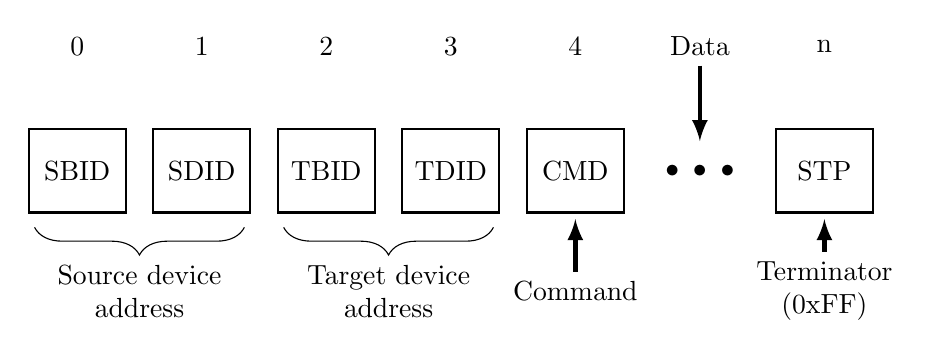
\begin{tikzpicture}[node distance=45pt,minimum size=1pt,auto]

\tikzstyle{pfield}=[rectangle,minimum width=35pt,minimum height=30pt,draw=black,thick];

\node [pfield] (b0) {SBID};
\node [pfield] (b1) [right of=b0] {SDID};
\node [pfield] (b2) [right of=b1] {TBID};
\node [pfield] (b3) [right of=b2] {TDID};
\node [pfield] (b4) [right of=b3] {CMD};

\node  (d0) [right of=b4,xshift=-10pt] {$\bullet$};
\node  (d1) [right of=d0,xshift=-35pt] {$\bullet$};
\node  (d2) [right of=d1,xshift=-35pt] {$\bullet$};

\node [pfield] (b5) [right of=d2,xshift=-10pt] {STP};

\draw [decorate,decoration={brace,amplitude=10pt,raise=5pt}] (b1.315) -- (b0.225) node [black,midway,align=center,yshift=-15pt] {\SDSTR};

\draw [decorate,decoration={brace,amplitude=10pt,raise=5pt}] (b3.315) -- (b2.225) node (t0) [black,midway,align=center,yshift=-15pt] {\TDSTR};

\node (t1) at (t0 -| b4) {\CMDSTR};
\node [align=center] (t2) at (t0 -| b5) {\TERMSTR \\ (0xFF)};

\path [-latex,ultra thick, shorten >=2pt] (t1) edge (b4);
\path [-latex,ultra thick, shorten >=2pt] (t2) edge (b5);

\node (t3) [above of=d1] {\DATASTR};

\path [-latex,ultra thick, shorten >=5pt] (t3) edge (d1);

%field number
\node [above of=b0] {0};
\node [above of=b1] {1};
\node [above of=b2] {2};
\node [above of=b3] {3};
\node [above of=b4] {4};
\node [above of=b5] {n};

\end{tikzpicture}
\end{document}